\section{Problem Details}
\label{problemdetails} 

%\begin{figure*}[ht]
\begin{figure}[ht]
		%[height=50mm,width=50mm]
		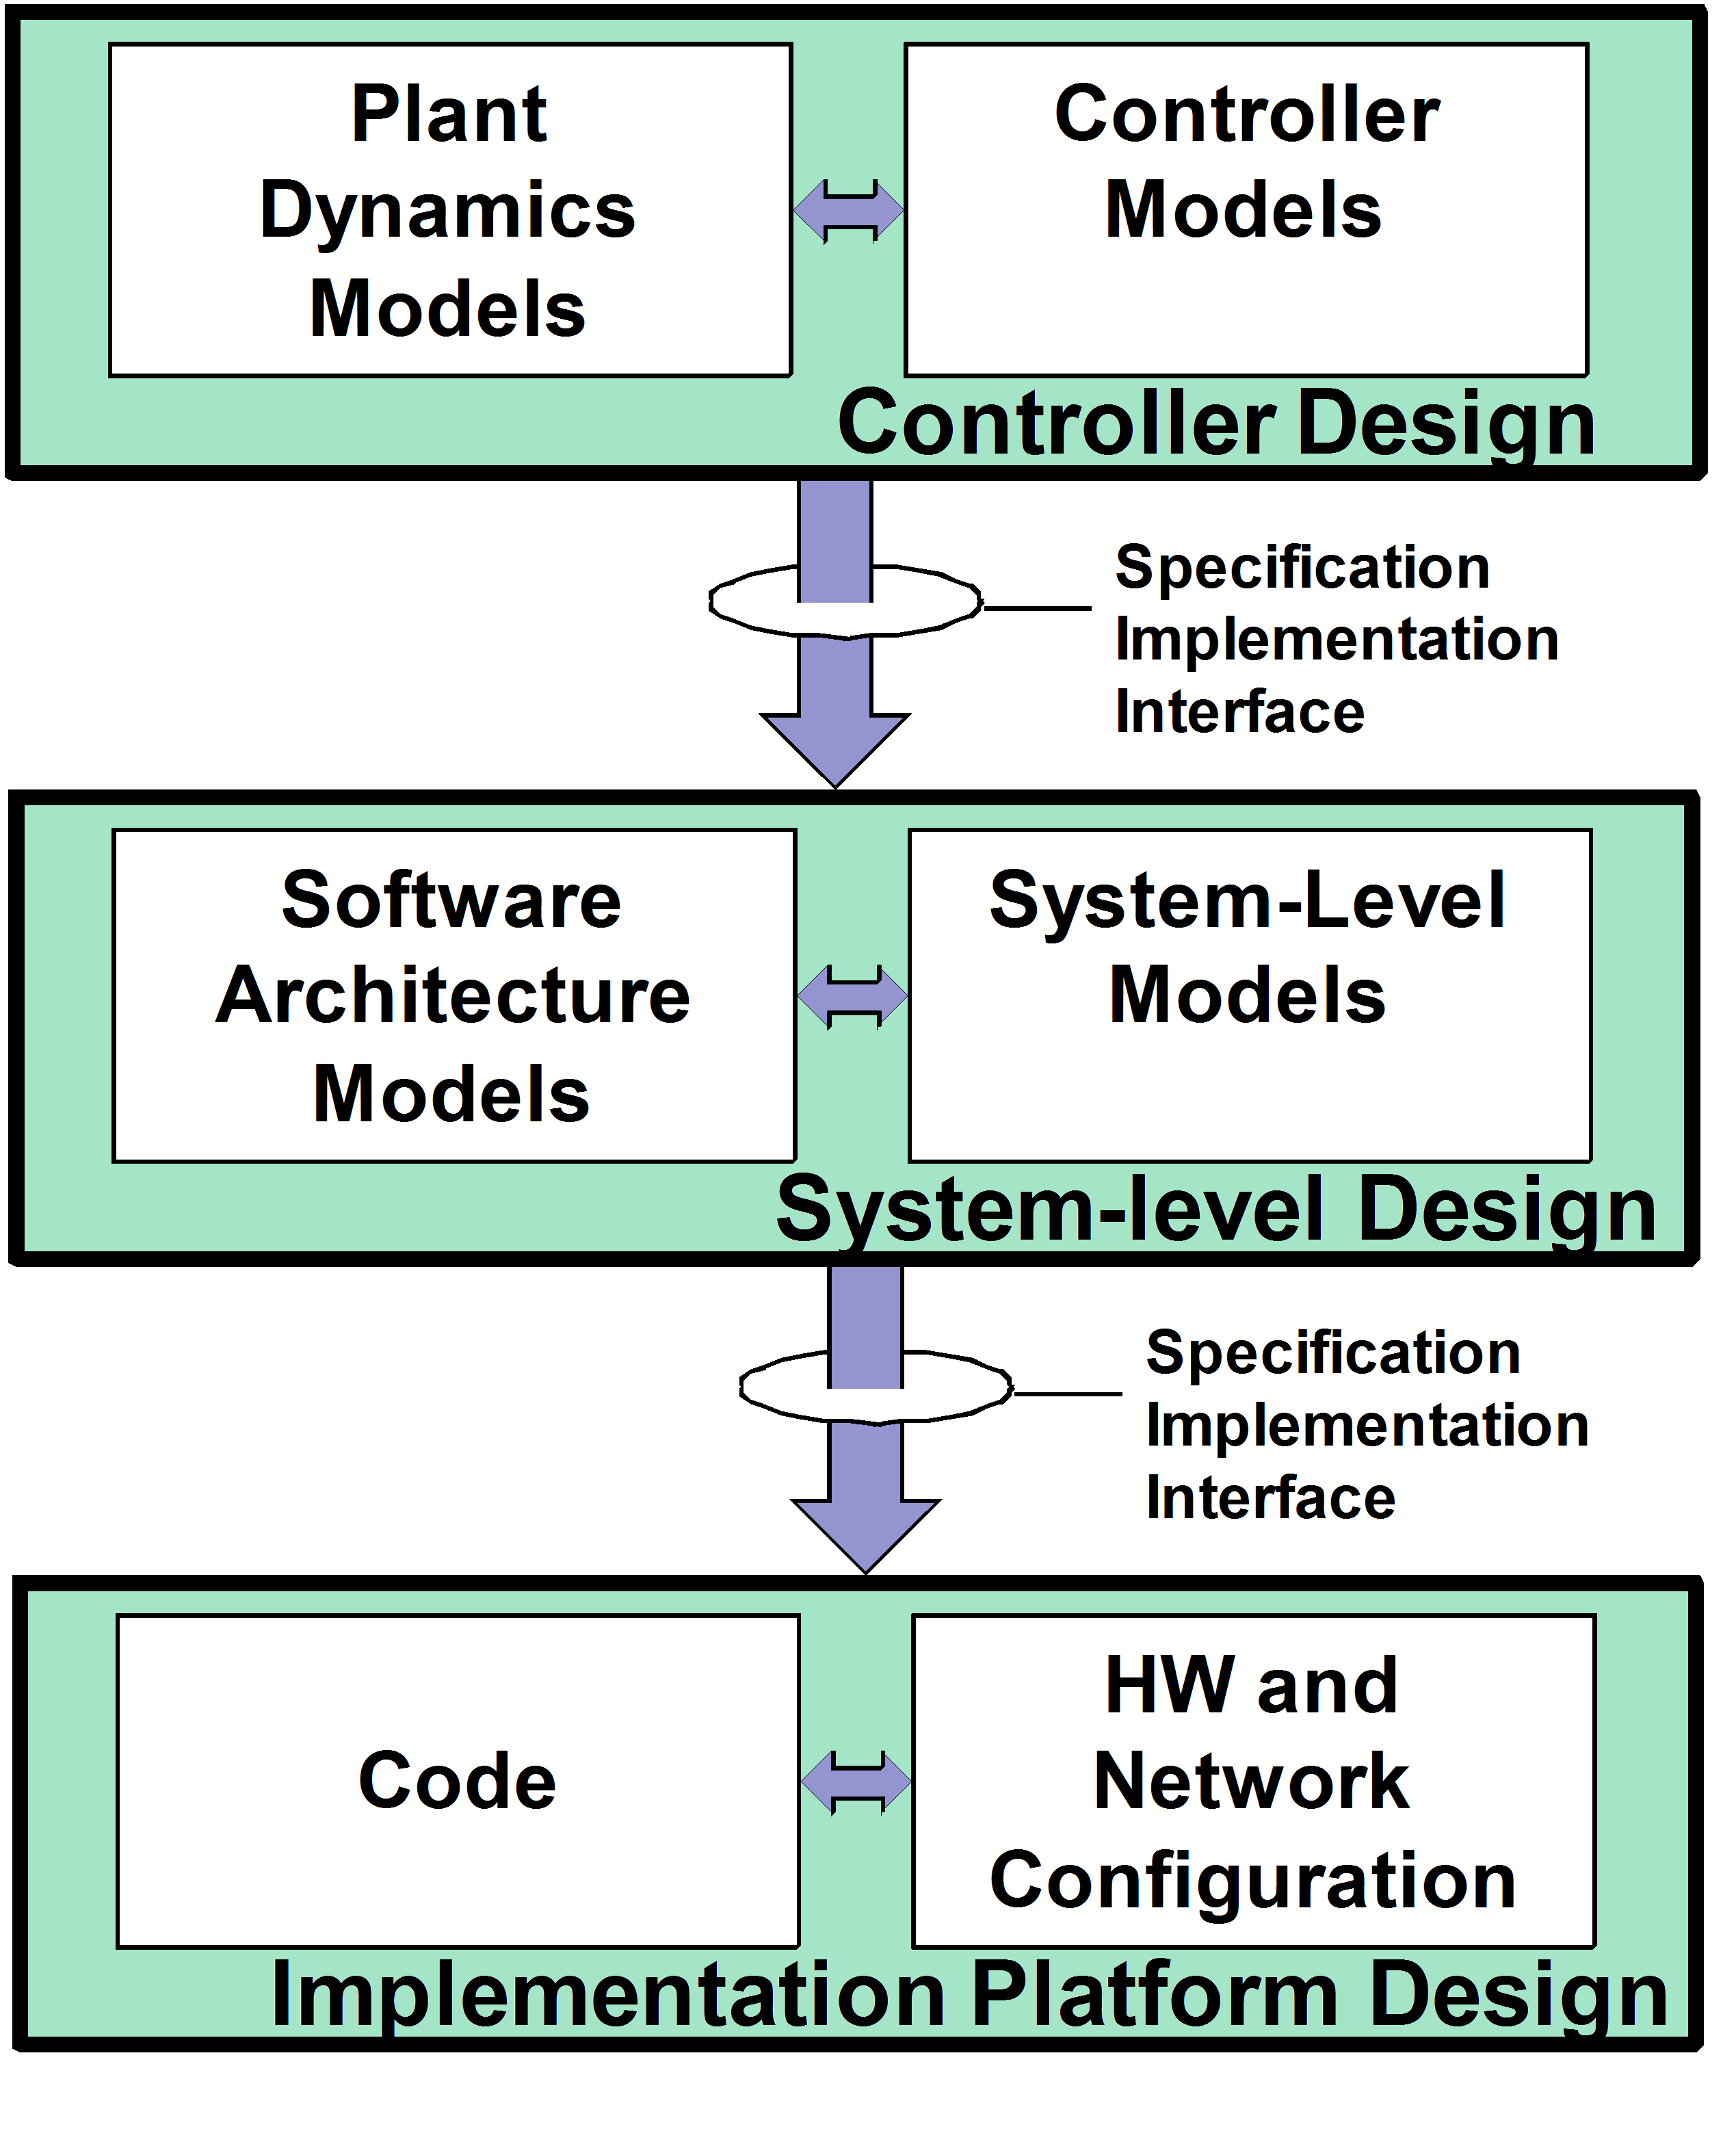
\includegraphics[scale=.4]{figures/design_diagram.png}
		\centering
	  \label{fig:design_diagram}
		\caption{Simplified Model-Based Design Flow}
\end{figure}

Model-based design and development have gained great traction in many computational domains.  Control designers create models for both physical systems and controllers using tools like Simulink and Stateflow from the Mathworks\cite{tools:mathworks}.  Design verification consists of simulated test cases and use of optimization tools to confirm stability and meet performance goals. Designers adjust parameters or redesign models to meet requirements.  Such models (and their supporting tools) correspond to the first stage in Fig. 1 (Controller Design). 

In the classical embedded systems design flow, control design models next pass to software developers (Fig. 1, System-level Design).  Software designers use models such as UML to specify platform details, code organization, and deployment configurations.  Timing is translated from the control specifications, and scheduling analysis is usually done during this stage.  Module developers may be given timing budgets to be satisfied.

The final development stage is software integration and testing on the deployed system (Fig. 1, Implementation Platform Design).  Engineers or software developers may perform integration and testing.  Designed control functions may exhibit new behavior when deployed on distributed architectures, or when code changes are made to address unanticipated problems (e.g., numerical precision, timing issues, etc...). Coupling between the control domain and the software design domain may first appear at this late stage of the process.  Designs which failed to account for coupled concerns in earlier stages may face costly redesigns.  In any case, late discovery of defects significantly increases cost \cite{prog:rapid_dev}.  In safety-critical NCS designs where defect counts must remain low, early defect detection is crucial.

Model-based design aims to support high-confidence embedded systems design by enabling exchange of information back along the development chain during design iterations.  For example, the extraction of useful information regarding problems found during scheduling analysis can enable rapid redesign of of control functions.  With respect to Fig. 1, this represents a flow of information against the normal development flow (counter to the arrows) during design iterations.  Fig. \ref{fig:flowchart} depicts such a development flow.  In order to support rapid model-based redesign, the models at different stages must contain abstractions of the platform execution effects.  For example, in scheduling this means that timing uncertainties introduced by the platform should be made available for use in scheduling models.  Even more useful is the ability to isolate scheduling problems and suggest processing rate adjustments to the control designers.  This contrasts with the usual yes-no results given by many constraint solvers.  In an ideal situation, a scheduling problem could be resolved by a control engineer and an embedded software engineer iterating design parameters and re-running the simulations and scheduling analysis together for an afternoon rather than a costly redesign later on.  It should be noted that this is a pattern for a solution -- as more kinds of model analysis enter the picture, this process increases in value.

\begin{figure}[ht]
		%[height=50mm,width=50mm]
		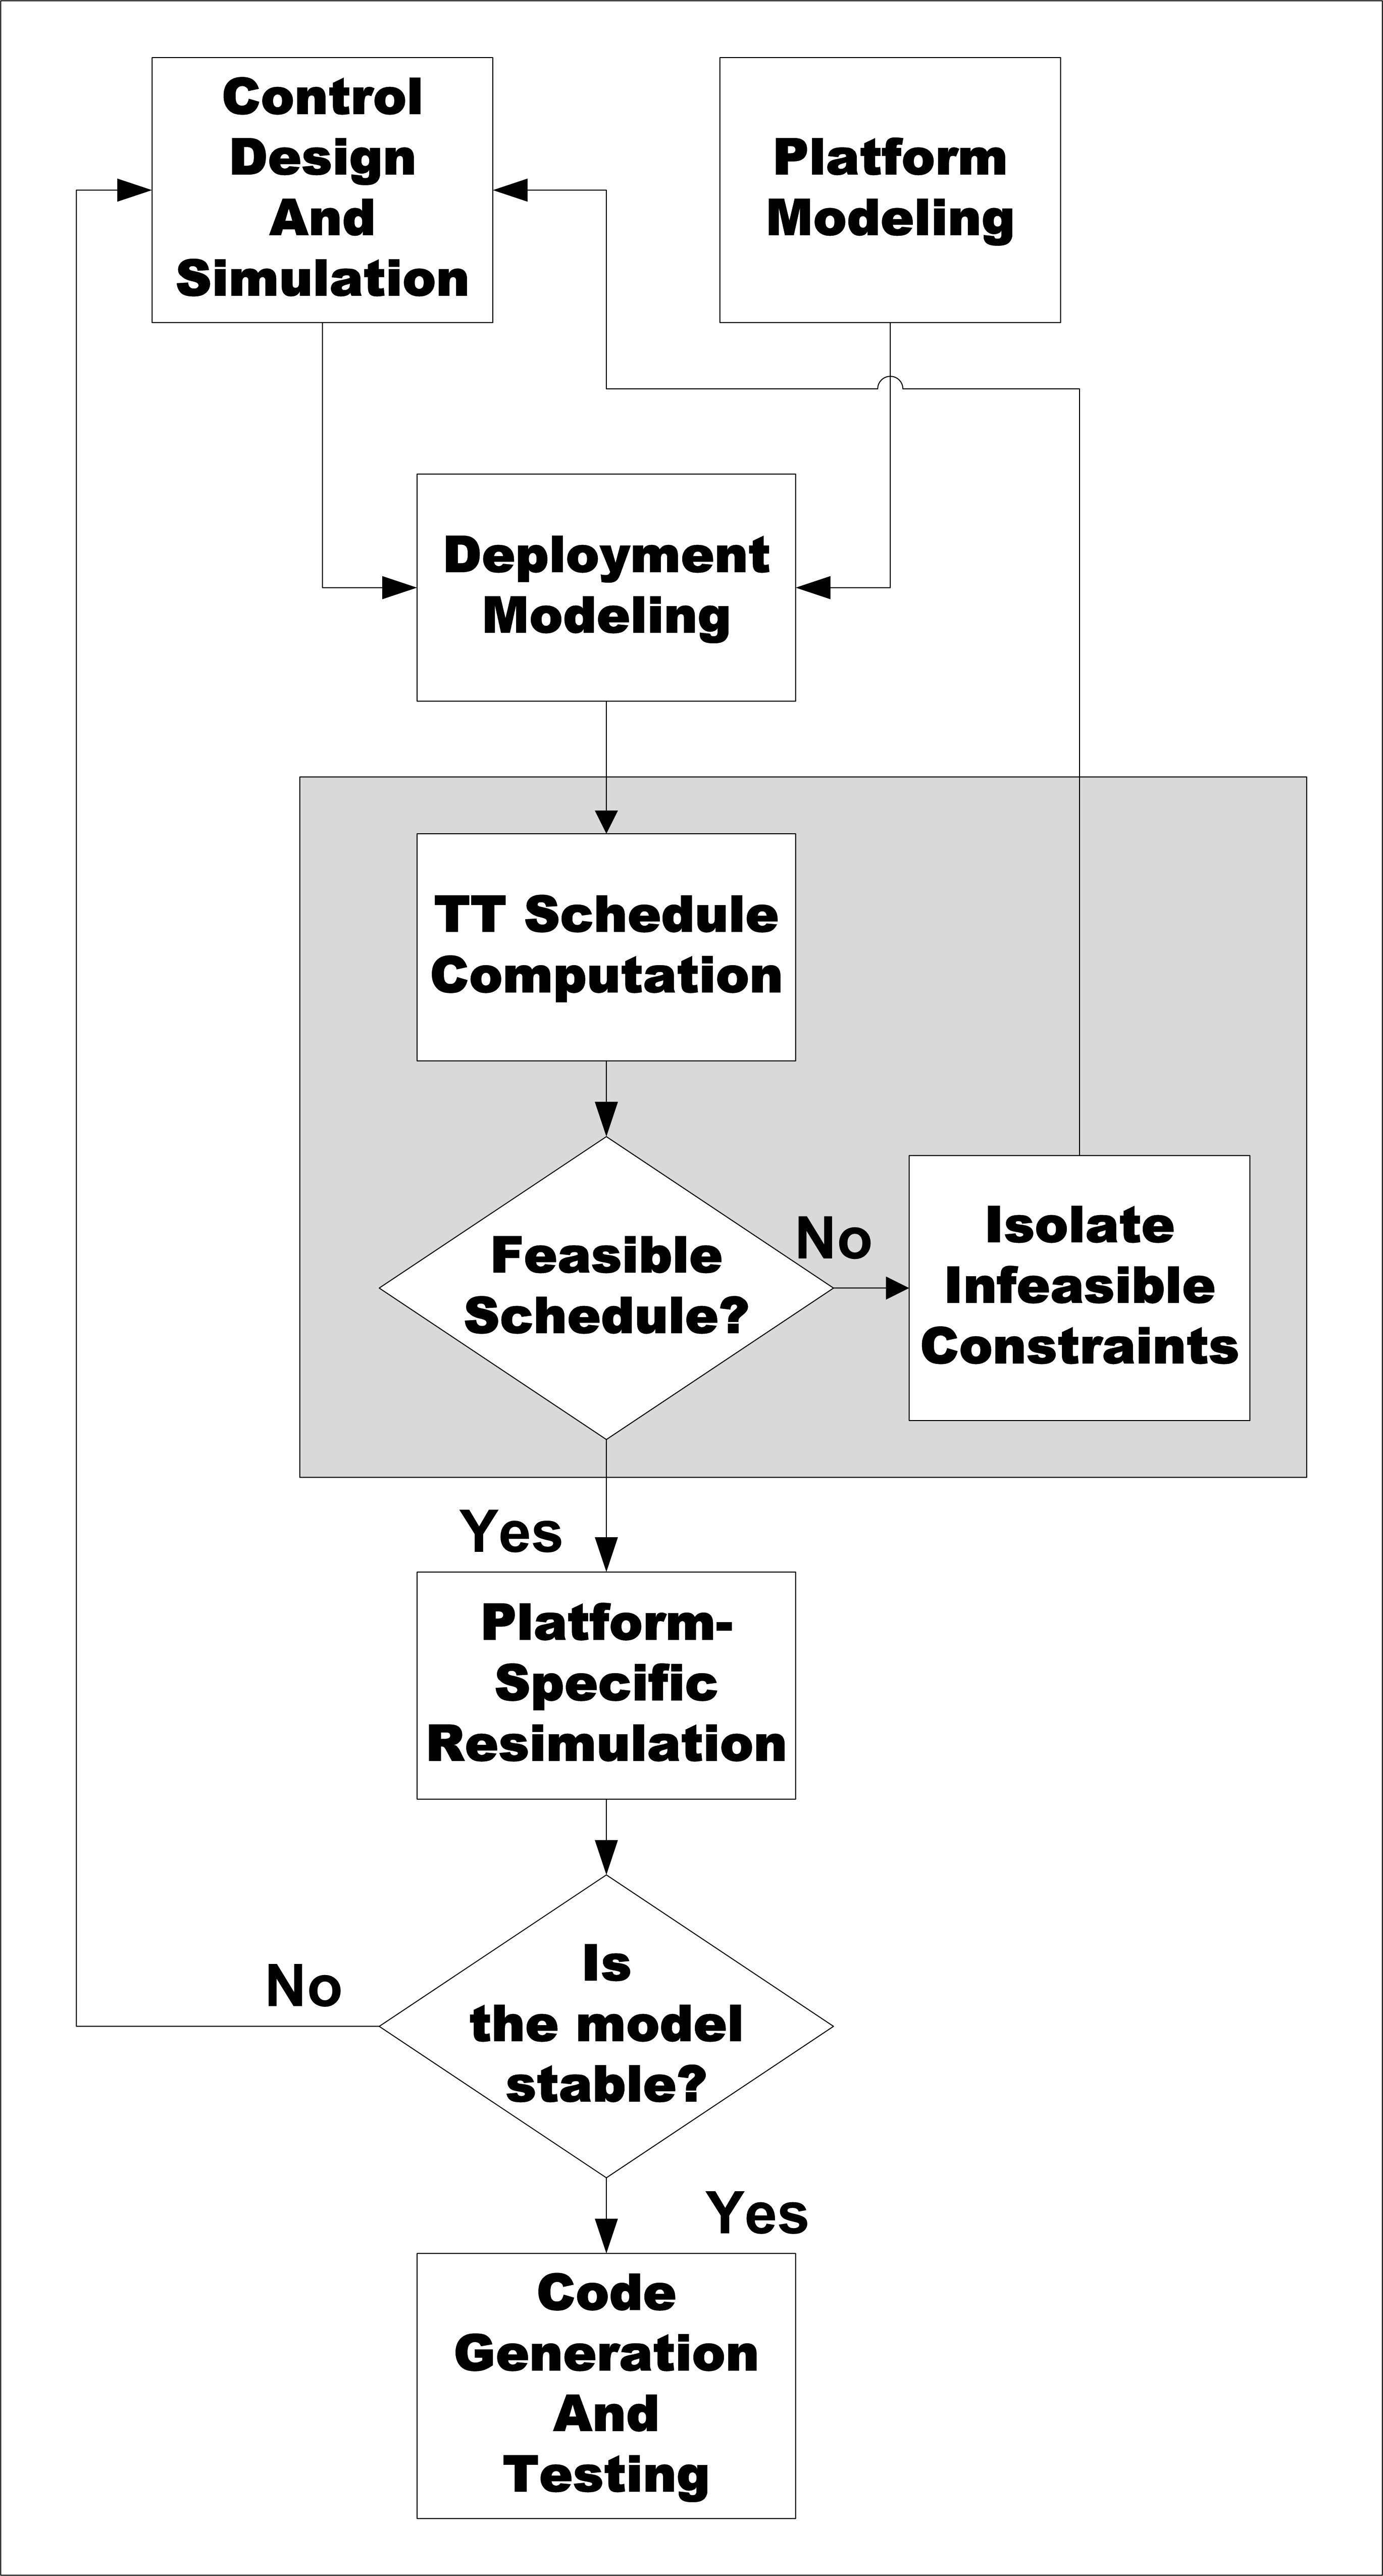
\includegraphics[scale=.6]{figures/flowchart.png}
		\centering
	  \label{fig:flowchart}
		\caption{Iterating a control design for platform function. The shaded box in the center highlights the scheduling steps addressed here.}
\end{figure}



